%-----------------------------------------------------------------------------
%
%               Template for sigplanconf LaTeX Class
%
% Name:         sigplanconf-template.tex
%
% Purpose:      A template for sigplanconf.cls, which is a LaTeX 2e class
%               file for SIGPLAN conference proceedings.
%
% Guide:        Refer to "Author's Guide to the ACM SIGPLAN Class,"
%               sigplanconf-guide.pdf
%
% Author:       Paul C. Anagnostopoulos
%               Windfall Software
%               978 371-2316
%               paul@windfall.com
%
% Created:      15 February 2005
%
%-----------------------------------------------------------------------------


\documentclass[preprint]{sigplanconf}

% The following \documentclass options may be useful:

% preprint      Remove this option only once the paper is in final form.
% 10pt          To set in 10-point type instead of 9-point.
% 11pt          To set in 11-point type instead of 9-point.
% authoryear    To obtain author/year citation style instead of numeric.

\usepackage{amsmath}
\usepackage{graphicx} 
\usepackage{color}
\usepackage{algpseudocode, algorithmicx, algorithm}
%\usepackage{ulem}
\usepackage{listings}
\usepackage{xcolor}
\usepackage{textcomp}

\newcommand{\op}[1]{\emph{#1}}
\newcommand{\descr}[1]{\emph{#1}}

\definecolor{teal}{RGB}{0,153,153}

\newcommand{\REVISE}[1]{\textcolor{red}{#1}}
\newcommand{\TODO}[1]{\textcolor{red}{#1}}
\newcommand{\NOTES}[1]{\textcolor{blue}{#1}}
\newcommand{\SVEN}[1]{\textcolor{green}{#1}}
\newcommand{\TY}[1]{\textcolor{teal}{#1}}
\newcommand{\STEVEN}[1]{\SVEN{\sout{#1}}}
\newcommand{\SYN}[1]{\textcolor{magenta}{#1}} %synonym
\long\def\/*#1*/{}
\begin{document}

\special{papersize=8.5in,11in}
\setlength{\pdfpageheight}{\paperheight}
\setlength{\pdfpagewidth}{\paperwidth}

\conferenceinfo{OOPSLA '14}{October 20--24, 2014, Portland, OR, USA} 
\copyrightyear{2014} 
\copyrightdata{978-1-nnnn-nnnn-n/yy/mm} 
\doi{nnnnnnn.nnnnnnn}

% Uncomment one of the following two, if you are not going for the 
% traditional copyright transfer agreement.

%\exclusivelicense                % ACM gets exclusive license to publish, 
                                  % you retain copyright

%\permissiontopublish             % ACM gets nonexclusive license to publish
                                  % (paid open-access papers, 
                                  % short abstracts)


\titlebanner{banner above paper title}        % These are ignored unless
\preprintfooter{short description of paper}   % 'preprint' option specified.

\title{A Simple and Scalable Wait-Free Ring Buffer}
%\subtitle{Subtitle Text, if any}

\authorinfo{Andrew Tyler Barrington}
           {University of Central Florida}
           {abarrington@knights.ucf.edu}
\authorinfo{Steven D. Feldman}
           {University of Central Florida}
           {feldman@knights.ucf.edu}
\authorinfo{Dr. Damian Dechev}
           {University of Central Florida}
           {dechev@eecs.ucf.edu}

\maketitle


\begin{abstract}
		% !TEX root = WaitFreeRingBuffer.tex

The ring buffer is a staple data structure in computer science applications.
In contrast to linked-list and vector data structures, ring buffers use a constant amount of memory.
This property makes it ideal for certain applications such as multimedia, network routing, trading systems, and gaming. 
In some of these cases, concurrent access is ideal or mandatory.
In this paper, we present a new non-blocking ring buffer that provides a wait-free progress guarantee suitable for such applications.

Several non-blocking queue implementations exist in the literature, however, we are not aware of any that provides the wait-free guarantee.
The design of efficient wait-free algorithms is challenging, because each thread operating on the data structure must complete its operation in a finite number of steps. 
This strict guarantee makes it ideal for real-time and mission critical systems, however, the added complexity to achieve this often results in reduced performance. \NOTES{revolutions in data memory (cite memsql)} %THIS NEEDS TO BE MADE BIG IMPACT
% CAN HELP THINGS LIKE MEMSQL

Circumventing such pitfalls, the presented concurrent ring buffer uses a methodology for diffusing contention, which results in a significant increase in performance.
Operating with 64 threads on a 64-core machine, performance results show that our algorithm performs on average X more operations than a coarse-grained locking approach, X more than TBB's concurrent bounded queue, and X more than the cycle queue by Tsigas.
\end{abstract}

\category{CR-number}{subcategory}{third-level}

% general terms are not compulsory anymore, 
% you may leave them out
\terms
term1, term2

\keywords
concurrent, non-blocking, wait-free, queue, ring buffer 

\section{Introduction}
		\label{sec:introduction}
		% !TEX root = WaitFreeRingBuffer.tex
The ubiquitous use of ring buffers in computer applications make them a focal point in computer science research.
A ring buffer or cyclical queue is a first-in-first-out queue that stores elements on a fixed length array.
In contrast to linked list queues, which do not have a maximum capacity, ring buffers are limited in capacity by the length of this array.
This array allows for efficient O(1) operations, cache-aware optimizations, and low memory overhead.
In general, the memory utilization of a ring buffer is limited to the cost of the array and two counters, making it desirable for systems with limited memory resources, such as embedded systems.

Ring buffers are found in a wide range of applications such as network routing, multimedia processing, and cloud-based services.
Many of these applications depend on ring buffers to pass work from one thread to another.
With the rise in many-core architectures, the number of threads executing in a system has greatly increased.
As a result, the efficiency of shared data structures, such as ring buffers, have a greater impact on performance than ever before.

In an attempt to achieve efficient and scalable performance, there has been significant research into the development of non-blocking algorithms.
These non-blocking algorithms forgo the use of locks, to permit greater scalability and core utilization.
Such designs are categorized by the level of progress they guarantee, with wait-free as the highest and most desirable categorization.
It provides freedom from deadlock, livelock, and thread starvation.
Deadlock is a result of multiple operations waiting on the other to finish, thus blocking all operations involved in the deadlock.
Livelock is similar to deadlock except operations yield to each other causing a lack of progress from the threads repeatedly making attempts to allow the other operation to progress.
Starvation occurs when an operation waits indefinitely for a resource~\cite{herlihy_bible}.
In addition to wait-free, non-blocking designs can also be categorized as either lock-free or obstruction-free.
In contrast to wait-free, lock-free designs are susceptible to thread starvation and obstruction-free designs are susceptible to both livelock and thread starvation~\cite{herlihy_bible}.

We are aware of two other non-blocking ring buffers in literatue.
Tsigas et al. presented a lock-free approach in which threads compete to apply an operation~\cite{tsigas}, however, this approach suffers from thread congestion and poor scaling.
Krizhanovsky presented a non-blocking approach which improves scalability through the use of the \emph{fetch and add} operation~\cite{?}, but unfortunately the design is susceptible to thread starvation and is not thread death safe.


We propose a new wait-free ring buffer algorithm based on the atomic \textit{fetch and add} (\emph{FAA}) operation.
A thread performing an enqueue or dequeue operation will perform a \emph{FAA} on the tail or head sequence counter, respectively.
The returned sequence identifier (\emph{seqid}) is used to determine the position to enqueue or dequeue an element from the buffer.
Specifically, the position is determined by the \emph{seqid} modulo the buffer's length.
To address the case where the \emph{seqid} of two different threads refer to the same position, we employ a novel method of determining which thread is assigned the position and which thread must get a new position.
To prevent the case where a thread is continually prevented from completing its operation, we integrated a progress assurance scheme~\cite{feldman_vector}.



The thread performing a dequeue operation will attempt to replace an element node whose \emph{seqid} matches its assigned \emph{seqid} with a newly allocated empty node.
This empty node's \emph{seqid} is equal to the current \emph{seqid} plus the length of the buffer.
Our restriction on the type of node a dequeue thread may remove, allows us to derive a FIFO\footnote{First in First Out} ordering of elements.
Without this restriction it is \textit{theoretically} possible for a thread to enqueue $A$ and $B$ and then dequeue $B$ followed by $A$, breaking the FIFO property.
We explain the specific scenario which may lead to this in Sec.~\ref{sec:todo}.
However, this restriction also introduces the scenario where if a thread never dequeues its node, then other threads with higher sequence numbers must wait.
If this scenario is detected, an atomic bitmark is placed on that value.
By using this bitmark, we can allow a dequeuer to get a new \emph{seqid} without the risk of an element being enqueued with the old \emph{seqid}.


Enqueueing threads will attempt to replace the current value with an element node, if the current value is an empty node whose \emph{seqid} is equal to the thread's \emph{seqid}.
If the current value has a \emph{seqid} less than the thread's \emph{seqid}, the thread will perform a back off routine to provide a delayed thread the opportunity to complete its operation.
If the current value has not changed, then depending on the node type (element or empty) and the \emph{seqid} (less than or greater), the thread will either get a new \emph{seqid} or replace the current node with its element node.
We explore the various states and their associated actions in Sec.~\ref{sec:todo}.

Previous research has shown that the use of the \emph{FAA} operation can provide significant increase in performance, when compared to similar designs implemented with the atomic compare-and-swap operation (\emph{CAS}).
For example, Feldman et al.~\cite{feldman_vector} compared the performance a \emph{FAA} based vector pushBack operation and a \emph{CAS} based approach and found that the \emph{FAA} design outperforms the \emph{CAS} design by a factor of 2.3.
This work includes a naive approach to designing a wait-free ring buffer using a multi-word compare-and-swap algorithm (MCAS)~\cite{feldman_mcas}.
This allows us to explore the performance difference between our \emph{FAA} based approach to that of a \emph{CAS} based approach.
Sec.~\ref{sec:mcasbuffer} provides a detailed analysis of the performance difference between these approaches.

We compare the performance of our implementation to that of other known concurrent ring buffers.
In this comparison, we explore how different distributions of operations, number of threads, and ring buffer size affect the throughput of each implementation.
On average, our design outperforms other designs by \% operations per second.
Compared to Intel Thread Building Blocks' concurrent bounded queue, we perform \% more operations per second.
Our results support our hypothesis that our design is scalable, making it optimal for many-core and real-time systems.

We provide the following novel contributions:
\begin{itemize}
\item To our knowledge this the first wait-free ring buffer.
Other known approaches, are susceptible to hazards such as live-lock and thread starvation.

\item Our design presents a unique way of applying sequence numbers and bitmarking to maintain provide the FIFO property.
This allows a simple way to mark and correct out-of-sync locations.


\item Our design maintains throughput in scenarios of high thread contention.
Other known approaches degrade as the thread contention increases, making it ideal for highly parallel environments.


\end{itemize}

\section{Related Works}
		\label{sec:related_work}
		% !TEX root = WaitFreeRingBuffer.tex

In this section we describe the implementation of other concurrent multiple producers and multiple consumers ring buffers.
%Though we are aware of several single producer and/or single consumer designs we do not discuss them.
%@Steven, it wont be considered bizzare having a single line introduction??

Tsigas~\cite{tsigas_queue} presents a lock free ring buffer in which threads compete to update the head and tail locations.
This design achieves dead-lock and live-lock freedom, but as we show in Sec.~\ref{sec:results}, this design scales poorly.
We attribute this poor performance to contention placed on head and tail locations.
The threads that fail their \op{CAS} operations are then forced to retry at the next location.
Some contention is reduced by lazily updating the head and tail references.
This requires an increased amount of read operations for threads to locate the actual index to operate, offsetting some contention.
%In our design we are able to reduce contention by forcing threads to update the head and tail values before performing their operation.
%@Andrew, I think it will be better to to do the comparison in Algorithm overview section
%@Steven, what comparison? I only contrast
%Fortunately, the \op{faa} operation used for this is both effecient and scalable~\cite{feldman_vector}.
%@Andrew, the above sentence is out of place and does not transition well. Look below for my example and either provide a better sentence or use it.

-%you can say: "This design achieves dead-lock and live-lock freedom, but the nature by which threads perform enqueueue and dequeue operations lead to poor performance in scenarios of high thread contention.
-%We attribute this poor performance to how the design only allows a single thread to succeed at completing an enqueue or dequeue operation, forcing other threads to retry."
-%Ending  like this, provides a good tie into the next FAA approach
%@Steven, are you saying cut the rest (remove starting at "Some contention is reduced..")? 

Tsigas~\cite{tsigas_queue} presents a lock free ring buffer in which threads compete to update the head and tail locations.
Enqueue is performed by determining the tail of the buffer and then enqueuing an element using a \op{cas} operation.
Dequeue is performed by determining the head of the buffer and then dequeueing the current element using a \op{cas} operation. 
This design achieves dead-lock and live-lock freedom, however, if a thread is unable to perform a successful \op{cas} operation, the thread will starve.
Unlike other designs, which are able to diffuse contention, the competitive nature of this design leads to increased contention and poor scaling.

Krizhanovsky~\cite{krizhanovsky_queue} presents a lock-free and high performance ring buffer.
This implementation, relies on the \op{faa} operation to increment head and tail counters, which assigns the location to perform an operation, thereby reducing thread contention and providing better scaling.
Each thread maintains a separate tail and head value of the index it last completed an enqueue or dequeue, respectively. 
The smallest of all threads' local head and tail values are used to determine the head and tail value at which all threads have completed their operations.
These values prevent operations from attempting to enqueue or dequeue at a location the previous operation has not yet completed.
Though this a non-blocking design, it is blocking in the case that if the buffer is empty or full, threads performing a dequeue or enqueue will wait until the buffer is not empty or not full, respectively.
%@Andrew say something about it not being thread death safe

The industry standard for many concurrent data structures is provided by Intel Thread Building Blocks (TBB)~\cite{tbb}.
This library provides a \emph{concurrent bounded queue} which utilizes a fine-grained locking scheme.
The algorithm uses an array of \emph{micro queue} to alleviate contention on individual indices.
Upon starting an operation, threads are assigned a ticket value which is used to determine sequence of operations in each \emph{micro queue}.
%@Andrew How are elements added to micro queues
If a threads ticket is greater than the expected, it will spin wait until the delayed threads have completed their operations.


%Optional Conclusion: (telling the reader what he was just told) if the next section needs a tie in
%@Andrew: Do a short compare/contrast to each
%For Tsigas: Like Krizzhanovsky's buffer we use the FAA to achieve better scalling and to reduce thread contnention
%Then say however in contrast to krizhanovsky, we are able to avoid the danger of live-lock, through how we manage our sequence number.
%Then say our design is composable with micro queue structures, and  then specify why it is different to a micro queue.
%This should be one flowing paragraph that shows progression from one to the next




\section{Restrictions and Limitations}
		\label{sec:restrictions}
		% !TEX root = WaitFreeRingBuffer.tex

Our approach requires the a sequentially consistent memory model to insure proper ordering of operations, as well as support for the atomic primitives \textit{compare and swap} (\op{cas}), \textit{fetch and add} (\op{faa}), \textit{fetch and or} (\op{fao}), \textit{load}, and \textit{store}.
Our design also reserves the least significant bit of a reference for state identification.

The presented implementation omits details related to memory management of short lived objects (i.e. \descr{Helper} and \descr{Node} objects).
The tested implementation uses a scheme based on the combination of hazard pointers~\ref{todo} and reference counting~\ref{todo} to prevent these objects from being reused prematurely.
Without such protection, it could introduce the ABA-problem~\ref{ABA}. 
For example, a thread could determine that it should replace a reference to a \descr{Node} object with a new \descr{Node} object.
However, before calling the \op{cas} operation, the object was removed and reallocated to another thread.
That thread, then placed the object at the same location it was removed from.
The first thread would be unaware that the contents of the \descr{Node} has changed, would incorrectly replace it.

For brevity and clarity, the pseudocode omits code related to the unbitmarking of references.
If a reference has been determined to hold a bitmark (i.e. \op{isSkipped} returning true), the next step would be to remove the bitmark from the local copy before dereferencing the object.

The use of the sequence identifiers introduces the \textit{theoretical} danger where the value rolls over, leading to two threads being assigned the same \emph{seqid}.
In the following algorithm discussions, we assume the sequence identifier does not have a maximum value and thus can not roll over.
The tested implementation uses a 64 bit signed long, which allows the ring buffer to support a maximum of $2^{63}$ enqueue operations.
In the event a roll over occurs, indicated by a negative result when incrementing a sequence counter, our implementation will creates a new internal ring buffer object where all subsequent elements are enqueued.
This is safe for systems using less than $2^{63}$ threads.

To achieve FIFO behavior of our ring buffer, we make the restriction that an element can only be dequeued by a thread whose \emph{seqid} matches the \emph{seqid} of the \descr{Node} containing the element.
To prevent the case where other threads maybe blocked in the event a dequeuer never removes its assigned element, we developed a method by which a thread is able to safely skip a position that holds a value assigned to another thread.

\section{Definitions and Structures}
		\label{sec:definitions}
		% !TEX root = WaitFreeRingBuffer.tex

Structures:
%Warning: Lstlisting does not ignore white space
\begin{itemize}

\item RingBuffer:
\begin{lstlisting}
{atomic array[],  atomic int head,
atomic int tail}
\end{lstlisting}

\item NullNode
\begin{lstlisting}
{const long seqid}
\end{lstlisting}

\item ElemNode
\begin{lstlisting}
{const long seqid, const Element element}
\end{lstlisting}

\item Helper
\begin{lstlisting}
{const Op *op, const long seqid, Node *old}
\end{lstlisting}

\item EnqueueOp
\begin{lstlisting}
{const Element, atomic Helper *helper}
\end{lstlisting}

\item DequeueOp
\begin{lstlisting}
{atomic Helper *helper}
\end{lstlisting}

\end{itemize}

Supporting Functions:
\TODO{Add 1-2 sentence descriptions}
\begin{itemize}
\item isNull():
\item isElement():
\item isSkipped():
\item setSkipped():
\item makeSkipped():
\item isHelper():
\item getNextTail():
\item getNextHead():
\item getPosition():
\item BackOff():
\end{itemize}



\subsection{Progress Assurance}
	\label{sec:definitions:progress_assurance}

For a design to be wait-free, a thread must not be continually denied access to a necessary resource.
This design employs a progress assurance scheme to prevent thread starvation.
Without this progress assurance scheme, the design presented may encounter a rare condition in which threads starve.
With larger ring buffer sizes, this possibility can be reduced further.

The progress assurance scheme is designed similar to the announcement table presented by Herlihy~\cite{herlihy_table}.
Threads will check the table incrementally at the start of every operation and help complete any operation found as presented by Kogan~\cite{kogan_fpsp}.
Our design is inpired by the design presented by Feldman, which is based on these two designs~\cite{feldman_vector}. % yes??
This design uses an announcement table of \emph{OpRec} which contains a \SYN{control word} indicating an operations state.
When the control word is a reference to a descriptor object the operation has been completed, otherwise, threads will continue to help.



\TODO{Describe it, cite Bible's Annoucement Table, Kogans method, Vector's Descriptor Association}

%What I want you to do is read the Progresss Assurance scheme section from my vector.
%Do a 5 sentences or less summary, then present a ring buffer specific implementation.

\section{Algorithm Overview}
		\label{sec:algorithm}
		% !TEX root = WaitFreeRingBuffer.tex

% !TEX root = WaitFreeRingBuffer.tex

\newcommand\fetchHead{
\begin{algorithm}[]
\caption{FetchHead $( )$ }
{\fontsize{8}{8}\selectfont
	\begin{algorithmic}[1]
		\State atomic\_fetch\_and\_increment(head)
	\end{algorithmic}
}
\label{alg:wf:example1}
\end{algorithm}
}

\newcommand\fetchTail{
\begin{algorithm}[]
\caption{FetchTail $( )$ }
{\fontsize{8}{8}\selectfont
	\begin{algorithmic}[1]
		\State atomic\_fetch\_and\_increment(tail)
	\end{algorithmic}
}
\label{alg:wf:example2}
\end{algorithm}
}

\newcommand\lfenqueue{
\begin{algorithm}[]
\caption{Enqueue $(val)$ }
{\fontsize{8}{8}\selectfont
	\begin{algorithmic}[1]
		\State TryHelpAnother()

		\State fail\_count = 0

		\While{true}
			\If {is\_full()} \label{alg:lf:enq:full}
				\State \Return false
			\EndIf

			\State seqid = next\_tail\_seq() \label{alg:enq:inc}
			\State pos = get\_position(seqid) \label{alg:enq:pos}
			\State  new\_node = new ElemNode(seqid, val) \label{alg:enq:elemnode}
			\While {true}
				\If {fail\_count++ $==$ MAX\_FAILS}
					\State op = new EnqueueOp(this, val)
					\State make\_announcement(op)
					\State \Return op.result()
				\EndIf

				\State node = buffer[pos].load()
				\If{node.op} \label{alg:enq:op}
					\State node.op.associate(node, \&(buffer[pos]))
					\State continue
				\ElsIf {isSkipped(node)} \label{alg:enq:bit}
					\State break
				\ElsIf {node.seqid $<$ seqid} \label{alg:enq:seqless}
					\State backoff()
					\If {node != buffer[pos].load()}
						\State continue
					\EndIf
				\EndIf

				\If {node.seqid $<=$ seqid  $and$ isEmpty(node)}
					\State success = buffer[pos].cas(node, new\_node) \label{alg:enq:common}
					\If {success}
						\State \Return true
					\EndIf
					\State continue
				\ElsIf {node.seqid $>$ seqid $or$ isElement(node)} \label{alg:enq:seqgreat}
					\State break
				\EndIf

			\EndWhile
		\EndWhile
	\end{algorithmic}
}
\label{alg:lf:enq}
\end{algorithm}
}

\newcommand\wfenqueue{
\begin{algorithm}[]
\caption{Wait-Free Enqueue $op$ }
{\fontsize{8}{8}\selectfont
	\begin{algorithmic}[1]
		\State seqid = get\_tail\_seq() -1
		\While{op.in\_progress()}
			\If {is\_full()}
				\State op.try\_set\_failed()
				\State \Return
			\EndIf

			\State seqid++
			\State pos = get\_position(seqid)
			\State  new\_node = new ElemNode(seqid, val, op)
			\While{op.in\_progress()}
				\State node = buffer[pos].load()
				\If{node.op}
					\State node.op.associate(node, \&(buffer[pos]))
					\State continue
				\ElsIf {isSkipped(node)}
					\State break
				\EndIf

				\If {node.seqid $<$ seqid}
					\State backoff()
					\If {node != buffer[pos].load()}
						\State continue
					\EndIf
				\EndIf

				\If {node.seqid $<=$ seqid  $and$ isEmpty(node)}
					\If {buffer[pos].cas(node, new\_node)}
						\State op.associate(new\_node, \&buffer[pos]);
						\State \Return
					\EndIf
				\ElsIf {node.seqid $>$ seqid $or$ isElement(node)}
					\State break
				\EndIf

			\EndWhile
		\EndWhile
	\end{algorithmic}
}
\label{alg:wf:enq}
\end{algorithm}
}


\newcommand\lfdequeue{
\begin{algorithm}[]
\caption{Dequeue $(\&result)$ }
{\fontsize{8}{8}\selectfont
	\begin{algorithmic}[1]
		\State TryHelpAnother()

		\State fail\_count = 0

		\While{true}
			\If {is\_empty()} \label{alg:lf:deq:empty}
				\State \Return false
			\EndIf

			\State seqid = next\_head\_seq() \label{alg:deq:inc}
			\State pos = get\_position(seqid) \label{alg:deq:pos}
			\State new\_node = new EmptyNode(seqid + capacity) \label{alg:deq:nullnode}
			\While{true}
				\If {fail\_count++ $==$ MAX\_FAILS} \label{alg:deq:maxfail}
					\State op = new DequeueOp(this)
					\State make\_announcement(op)
					\State \Return op.result(result)
				\EndIf

				\State node = buffer[pos].load()

				\If{node.op} \label{alg:deq:op}
					\State node.op.associate(node, \&(buffer[pos]))
					\State continue
				\ElsIf {isSkipped(node) $and$ isEmpty(node)} \label{alg:deq:fix}
					\If {buffer[pos].cas(node, new\_node)}
						\State break
					\Else
						\State continue
					\EndIf
				\ElsIf {seqid $ > $ node.seqid} \label{alg:deq:seqless}
					\State backoff()
					\If {node $==$ buffer[pos].load()}
						\If {isEmpty(node)}
							\If {buffer[pos].cas(node, new\_node)}
								\State break
							\EndIf
						\Else
							\State atomic\_mark\_skip(\&buffer[pos])
						\EndIf
					\EndIf
				\ElsIf {seqid $ < $ node.seqid} \label{alg:deq:seqgreat}
					\State break
				\Else % is not owned
					\If {isElem(node)}
						\If {isSkipped(node)}
							\State new\_node = setSkipped(new\_node)
						\EndIf
						\State success = buffer[pos].cas(node, new\_node) \label{alg:deq:common}
						\If {success}
							\State *result = node.value
							\State \Return true
						\EndIf
					\Else \label{alg:deq:nullnode}
					%isEmpty(node)
						\State backoff()
						\If {node $==$ buffer[pos].load()}
						 	\If {buffer[pos].cas(node, new\_node)}
								\State break
							\EndIf
						\EndIf
					\EndIf
				\EndIf

			\EndWhile
		\EndWhile
	\end{algorithmic}
}
\label{alg:lf:deq}
\end{algorithm}
}


\newcommand\wfdequeue{
\begin{algorithm}[]
\caption{Wait-Free Dequeue $(op)$ }
{\fontsize{8}{8}\selectfont
	\begin{algorithmic}[1]
		\State seqid = get\_head\_seq() -1
		\While{op.in\_progress()}
			\If {is\_empty()}
				\State \Return op.try\_set\_failed()
			\EndIf

			\State seqid++
			\State pos = get\_position(seqid)

			\While{op.in\_progress()}

				\State node = buffer[pos].load()

				\If{node.op}
					\State node.op.associate(node, \&(buffer[pos]))
					\State continue
				\ElsIf {isSkipped(node)}
					\If {isEmpty(node)}
						\If {buffer[pos].cas(node, new\_node) == false}
							\State continue
						\EndIf
					\EndIf
					\State break
				\Else %curr_node is not skip-marked
					\If {seqid $<$ node.seqid}
						\State backoff()
						\If {node $==$ buffer[pos].load()}
							\State break
						\EndIf
					\ElsIf {sec $>$ node.seqid}
						\State break
					\Else % seqid == node.seqid
						\If {isElem(node)}
							\State new\_node = new ElemNode(seqid, node.value, op)
							\If {buffer[pos].cas(node, new\_node)}
								\State op.associate(new\_node, \&(buffer[pos]))
								\State \Return
							\EndIf
						\Else
							\State break
						\EndIf
					\EndIf
				\EndIf
			\EndWhile
		\EndWhile
	\end{algorithmic}
}
\label{alg:wf:deq}
\end{algorithm}
}


\newcommand\dequeueassoc{
\begin{algorithm}[]
\caption{DequeueOp::associate $(node, address)$ }
{\fontsize{8}{8}\selectfont
\begin{algorithmic}[1]
	\State success = helper.cas(null, node) \label{alg:deq:assoc:lin}
	\If {success $or$ helper.load() == node}
		\State new\_node = NullNode(node.seqid + capacity)
		\If{address.cas(node,  new\_node) == false}
			\State node = setSkipped(node)
			\If{address.load() == node}
				\State new\_node = setSkipped(new\_node)
				\State address.cas(node,  new\_node)
			\EndIf
		\EndIf
	\Else
		\State node.op.store(null);
	\EndIf
\end{algorithmic}
}
\label{alg:deq:assoc}
\end{algorithm}
}

\newcommand\enqueueassoc{
\begin{algorithm}[]
\caption{EnqueueOp::associate $(node, address)$ }
{\fontsize{8}{8}\selectfont
\begin{algorithmic}[1]
	\State success = helper.cas(null, node)
	\If {success $or$ helper.load() == node}
		\State node.op.store(NULL)
	\Else
		\State new\_node = NullNode(node.seqid)
		\If{address.cas(node,  new\_node) == false}
			\State node = setSkipped(node)
			\If{address.load() == node}
				\State new\_node = setSkipped(new\_node)
				\State address.cas(node,  new\_node)
			\EndIf
		\EndIf
	\EndIf
\end{algorithmic}
}
\label{alg:enq:assoc}
\end{algorithm}
}
\newcommand\opTryFail{
\begin{algorithm}[]
\caption{Op::try\_set\_failed $()$ }
{\fontsize{8}{8}\selectfont
\begin{algorithmic}[1]
	\State helper.cas(null, FAIL) \label{alg:op:tryfail:lin}
\end{algorithmic}
}
\label{alg:op:tryfail}
\end{algorithm}
}

\newcommand\template{
\begin{algorithm}[]
\caption{template $(operand)$ }
{\fontsize{8}{8}\selectfont
\begin{algorithmic}[1]

\end{algorithmic}
}
\label{alg:template}
\end{algorithm}
}

%\lstset{
%  basicstyle=\small\singlespace,
%  morekeywords={const, atomic}
%}

In this section, we first present an overview of our approach, and then describe our specific implementation of the enqueue and dequeue operations.

In contrast to designs in which threads compete to finish an operation, our approach diffuses thread contention and reduces \SYN{forced dependency}.
We accomplish this through the use of sequence counters to \SYN{assign} order to threads performing enqueue and dequeue operations.
The presented implementation stores references \SYN{to} (\TY{of}) \descr{Node} objects in the ring buffer.
As described in Sec.~\ref{sec:definitions}, \descr{Node} objects contain a \emph{seqid} member, and if its is an \descr{ElemNode} it also contains an element member.
The position at which a \descr{Node} reference is placed, is determined by performing a mod operation on the \emph{seqid} using the length of the ring buffer.

Our implementation solves several dangers that may arise by using this methodology.
The first, is the case where an enqueue thread is assigned a position, but an \descr{ElemNode} already exists at that position.
The second, is the case where a dequeuer thread is assigned a position, but an \descr{EmptyNode}  exists at that position.
And a third danger, is the case where a dequeuer thread is assigned a position that holds a value, but its \emph{seqid} is less than the thread's \emph{seqid}.
These dangers can arise as a result of poor system scheduling, \SYN{inopportune} context switches, and thread delay. % @Steven, the examples are different but seem similar and redundant IMO
Our implementations include a novel solution that uses the atomic fetch and or (\op{fao}) operation along with the \emph{seqid} to ensure that these dangers do not affect the correctness of our implementation.


The remainder of this section is structured as follows:
We present a detailed explanation of enqueue and dequeue operations.
This explanation includes algorithm \SYN{behavior}, linearizability, and wait-freedom descriptions.
Next, provide several case examples using Figs.~\ref{todo} to describe several execution scenarios.
\SYN{After which}, we present an informal reasoning on algorithm correctness and linearizability.


\begin{figure*}[ht!]
\centering
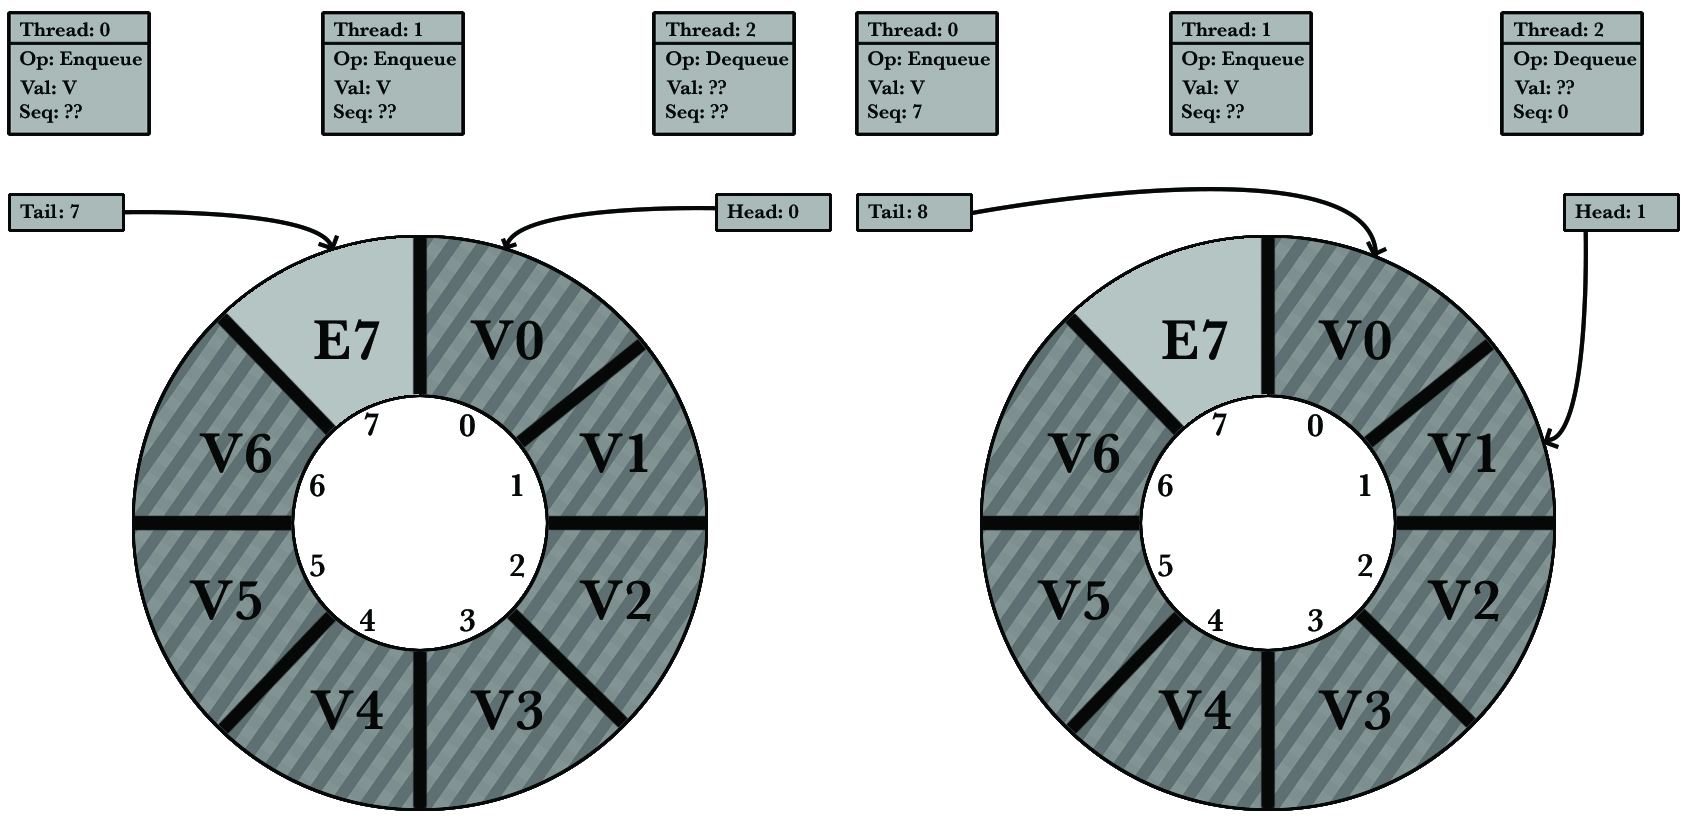
\includegraphics[width=90mm]{figures/buffer_init.jpg}
\caption{Init}
\label{buffer_ex}
\end{figure*}

\begin{figure}[ht!]
\centering
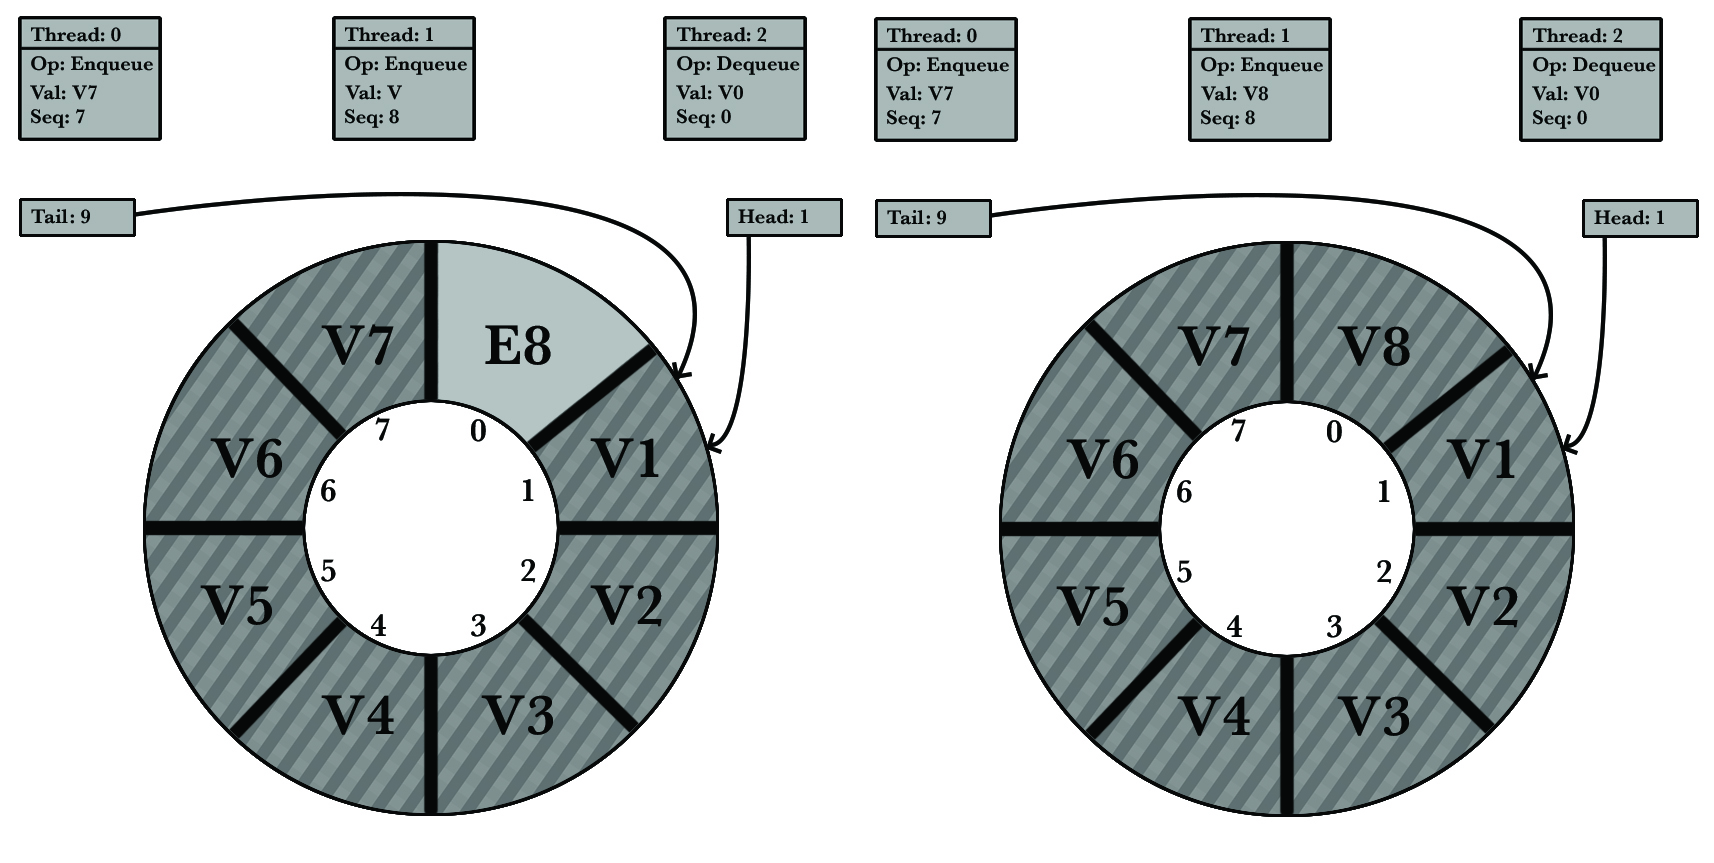
\includegraphics[width=90mm]{figures/buffer_ideal.jpg}
\caption{Ideal}
\label{buffer_ex}
\end{figure}

\begin{figure}[ht!]
\centering
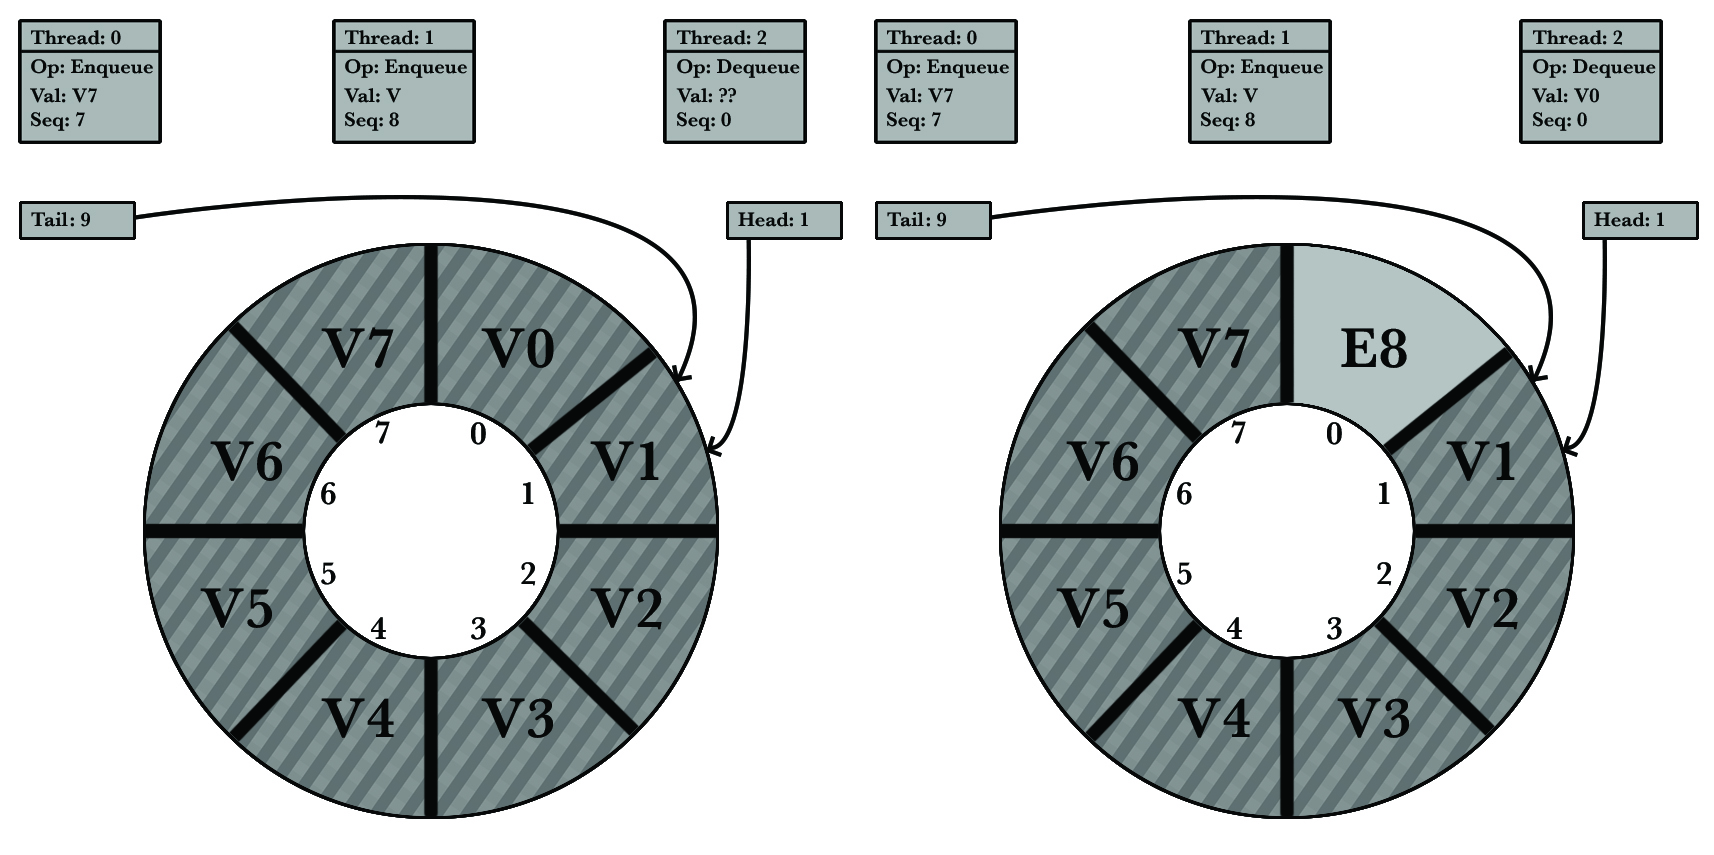
\includegraphics[width=90mm]{figures/buffer_full.jpg}
\caption{Full}
\label{buffer_ex}
\end{figure}


% ==============================
\section{Dequeue} % =========
\label{sec:alg:deq}
% ==============================

% =~=~=~=~=~=~=~=~=~=~=~=~=~=~=~
\lfdequeue % =~=~=~=~=~=~=~=~=~=
\wfdequeue % =~=~=~=~=~=~=~=~=~=
\opTryFail
\dequeueassoc % =~=~=~=~=~=~=~=~=~=


The following describes how a dequeue operation is performed. % @Steven, shouldnt this be implied enough by the section header and if not it seems a bit blunt
To guide the reader, we reference specific lines in Alg.~\ref{alg:lf:deq}

To \op{dequeue} an element, a thread will first check if the ring buffer is empty (L.~\ref{alg:lf:deq:empty}), returning false if it is.
Otherwise, it will acquire a dequeue sequence number, \emph{seqid}, from the head counter and determine the position, \emph{pos}, to dequeue an element (L.~\ref{alg:deq:inc}-~\ref{alg:deq:pos}).
The thread will then prepare an \descr{EmptyNode} to replace the dequeued value (L.~\ref{alg:deq:EmptyNode}). % @Steven, are we going back this route? you told me before to change the code to be as local with its usage as possible with the EmptyNode preaparation
The \emph{seqid} of the \descr{EmptyNode} is set to the assigned \emph{seqid} plus the buffer's capacity.
In the common case,  the thread will replace an \descr{ElemNode}, whose \emph{seqid} matches its assigned \emph{seqid}, with the prepared \descr{EmptyNode} (L.~\ref{alg:deq:common}).
Uncommon cases, which are often the result of thread delay, are described below.


\begin{itemize}
\item The node holds a reference to an operation record (L.~\ref{alg:deq:op}).
This indicates the node was placed as part of another thread's operation.
The thread will call the associate function for that operation and upon its return either the node has been replaced or the reference to the operation record has been removed.
The node at the current position will then be re-examined.

\item The node currently at the position has a \emph{seqid} number less than the assigned or it is an \descr{EmptyNode} \emph{seqid}(L.~\ref{alg:deq:seqless}, L.~\ref{alg:deq:EmptyNode}).
In this event, we call the backoff routine to provide an opportunity for a delayed thread to complete its operation.
If the current node has not changed the thread will advance the position by either replacing an \descr{EmptyNode} with the prepared \descr{EmptyNode} or performing an atomic bitmark if it is an \descr{ElemNode}.
If the node has changed, the position will be re-examined.

In order to achieve FIFO ordering, threads can only remove an \descr{ElemNode} if it was assigned that node's \emph{seqid}.
The atomic bitmark allows a thread to get a new \emph{seqid} without the risk of an \descr{ElemNode} being enqueued with a \emph{seqid} that has been given up. % @Steven, we should work to make this more clear when we revise together

\item The node currently at the position is bitmarked and an \descr{EmptyNode} (L.~\ref{alg:deq:fix}).
This state resulted from the previously described, in which a thread bitmarked an \descr{ElemNode}.
The thread who was assigned that node's \emph{seqid} must have replaced it with a bitmarked \descr{EmptyNode}.
Sec.~\ref{sec:correctness} describes the importance of replacing a bitmarked \descr{ElemNode} with a bitmarked \descr{EmptyNode}.
This state is resolved by replacing  the bitmarked \descr{EmptyNode} with  an unbitmarked \descr{EmptyNode}.

\item The node currently at the position has a \emph{seqid} greater than the assigned \emph{seqid} (L.~\ref{alg:deq:seqgreat}).
This implies that some thread caused this thread's \emph{seqid} to be skipped and as result this thread needs to get a new \emph{seqid}.

\end{itemize}

% @Steven, I feel the new code is well described but the flow and structure of the code itself makes it more difficult to follow. I also think with the progress assurance that follows this, I think it gives the impression the code heavily relies on the progress assurance to achieve wait-freedom rather than in the last structure it seemed easier to see the rarity. But after reading enqueue Ive slightly changed my mind

These uncommon cases could force a thread to indefinitely reattempt its operation.
However, we employ a progress assurance scheme to prevent this from occurring.
Specifically, in the event a threshold is reached (L.~\ref{alg:deq:maxfail}) the thread will make an announcement and switch to a slow path dequeue operation (Alg.~\ref{alg:wf:deq}). We describe in Sec.~\ref{sec:progressassurance}, specifically how this announcement scheme is used to ensure an operation is completed in a finite number of steps.

The wait-free dequeue operation functions very similarly to the normal dequeue operation with the following key change.
\begin{itemize}
\item The operation ends when some threads calls either \emph{op.try\_set\_failed} or \emph{op.associate}.
Upon return of these functions it is guaranteed that the operation has been completed.
\item The thread is not assigned a \emph{seqid} but instead loads the current value of the head counter.
This is important to prevent the scenario where a thread is assigned a position after the operation has been completed and as a result no longer needs to dequeue a value.
\item The node placed holds a reference to the operation record it was placed on behalf of.
This is used to prevent the case where multiple threads complete the same operation.
Multiple nodes may reference the same operation record, but the operation record may only refence one of these nodes: the completed operation.
\item After a node is placed, the operation's associate function is called.
This ensures that if the node was placed incorrectly its reference to the operation record will be removed.
If it was placed correctly, then the node will be replaced by an \descr{EmptyNode}.

\end{itemize}


\subsection{Linearizability}
In general the linearization point for a successful dequeue operation is the atomic \op{faa} operation which assigned the \emph{seqid} (L.~\ref{alg:deq:inc}).
However, this is not realized until the thread successfully places an \descr{EmptyNode} in place of the \descr{ElemNode} with \emph{seqid} matching the \emph{seqid} assigned (L.~\ref{alg:deq:common}).
If the wait-free path is used then the linearization point for a successful dequeue operation is the successful association of an \descr{ElemNode} and a \descr{DequeueOp} (Alg.~\ref{alg:deq:assoc} L.~\ref{alg:deq:assoc:lin}).

The linearization point for a failed dequeue operation is when a thread thread detects that the ring buffer is empty  (Alg.~\ref{alg:lf:deq} L.~\ref{alg:lf:deq:empty}).

If the wait-free path is used then the linearization point for a failed dequeue operation is the successful \op{cas} that set the operation's \emph{helper} member to the \emph{FAIL} constant (Alg.~\ref{alg:op:tryfail} L.~\ref{alg:op:tryfail:lin}).


% ==============================
\section{Enqueue} % =========
\label{sec:alg:dequeue}
% ==============================

% =~=~=~=~=~=~=~=~=~=~=~=~=~=~=~
\lfenqueue % =~=~=~=~=~=~=~=~=~=
\wfenqueue % =~=~=~=~=~=~=~=~=~=
\enqueueassoc % =~=~=~=~=~=~=~=~=~=
% =~=~=~=~=~=~=~=~=~=~=~=~=~=~=~

The following describes how a enqueue operation is performed.
To guide the reader, we reference specific lines in Alg.~\ref{alg:lf:enq}

To \op{enqueue} an element, a thread will first check if the ring buffer is full (L.~\ref{alg:lf:enq:full}), returning false if it is.
Otherwise, it will acquire a enqueue sequence number, \emph{seqid}, from the tail counter and determine the position, \emph{pos}, to enqueue an element (L.~\ref{alg:enq:inc}-~\ref{alg:enq:pos}).
The thread will then prepare an \descr{ElemNode} to hold the element being enqueued (L.~\ref{alg:enq:elemnode}).
The \emph{seqid} of the \descr{ElemNode} is set to the assigned \emph{seqid}.
In the common case,  the thread will replace an \descr{EmptyNode}, whose \emph{seqid} matches its assigned \emph{seqid}, with the prepared \descr{ElemNode} (L.~\ref{alg:enq:common}).
Uncommon cases, which are often the result of thread delay, are described below.

\begin{itemize}
\item The node holds a reference to an operation record (L.~\ref{alg:enq:op}).
This indicates the node was placed as part of another thread's operation.
This must be resolved by calling the associate function for that operation.
Upon its return either the node has been replaced or the reference to the operation record has been removed.
The thread will then re-examine the current position.

\item The reference currently at the position has a bitmark (L.~\ref{alg:enq:bit}), indicating it was marked as skipped.
This indicates the node at the position needs to be fixed by a dequeue thread.
As a result, the enqueue thread will get a new \emph{seqid} and retry its operations.

\item The node currently at the position has a \emph{seqid} number less than the assigned the \emph{seqid} (L.~\ref{alg:enq:seqless}).
In this event,the thread will call the backoff routine to provide time for a delayed thread to complete its operation.
If the current node has not changed and it is an \descr{EmptyNode} the thread will attempt to replace it with the prepared \descr{ElemNode}.
Otherwise, it will get a new \emph{seqid}.

\item The node currently at the position has a \emph{seqid} greater than the assigned \emph{seqid} (L.~\ref{alg:enq:seqgreat}).
This implies that some thread caused this thread's \emph{seqid} to be skipped and as result this thread needs to get a new \emph{seqid}.

\end{itemize}

As described in Sec.~\ref{sec:alg:dequeue}, these uncommon cases could force a thread to indefinitely reattempt its operation.
The following are key differences between the normal enqueue operation and the wait-free enqueue operation.
\begin{itemize}
\item The operation ends when some threads calls either \emph{op.try\_set\_failed} or \emph{op.associate}. % line 4, 13, 26
Upon return of these functions it is guaranteed that the operation has been completed.
\item The thread is not assigned a \emph{seqid} but instead loads the current value of the tail counter.
This is important for achieving maximum unskipped buffer indices resulting from cancelled operations.
%This is important to prevent the scenario where a thread is assigned a position after the operation has been completed and as a result no longer needs to enqueue a value.
\item The node placed holds a reference to the operation record it was placed on behalf of.
This is used to prevent the case where multiple threads complete the same operation.
Many nodes may reference the same operation record, but the operation record may only refence one of these nodes: the completed operation.
\item After a node is placed, the operation's associate function is called.
This ensures that if the node was placed incorrectly then the node will be replaced by an \descr{EmptyNode}.
If it was placed correctly, its reference to the operation record will be removed.

\end{itemize}

\section{Wait-Freedom}
We show that both the dequeue and enqueue algorithms are wait-free by first examining the loops and their terminating conditions. Both algorithms contain two nested while loops and in general the outer loop executes until the operation has been completed and the inner loop executes until the assigned \emph{seqid} is no longer viable.
The \emph{MAX\_FAILS} constant is used to place an upper bound on the number of times a thread will execute these loops.
If this constant is reached, \op{make\_announcement} is called and be our definition of this function upon its return the operation must be complete. Thus if all functions called by \op{dequeue} or \op{enqueue}, then these functions are wait-free.


Except for  \op{TryHelpAnother} and \op{make\_announcement}, the functions called are utility functions that are used to simplify the code explanation.
These functions are inherently wait-free because they contain no loops or calls to non-wait-free functions.
However, both \op{TryHelpAnother} and \op{make\_announcement} are capable of calling \op{wait-free dequeue} or \op{wait-free enqueue}, thus wait-freedom is determined by the progress guarantee of these two operations.

Both \op{wait-free dequeue} or \op{wait-free enqueue} employ the same looping structures which terminate when the operation record (\emph{op}) is no longer in progress. An operation record is in progress as long as its \emph{helper} member is \emph{null}.
\TODO{discuss how its lf and blah blah and if it enough operations occur, all threads will be helping, thus it is wait-free...}


\section{Correctness}
		\label{sec:correctness}
		% !TEX root = WaitFreeRingBuffer.tex

% when you use quotes in Latex you should start with `` and end with " -- this indicates good style

\newtheorem{lemma}{Lemma}
\newtheorem{theorem}{Theorem}

This section presents an informal proof that the ring buffer is correct.
It is divided into three parts; the first two we present an informal proof that shows the enqueue and dequeue operations behave as described and the third part shows that the buffer provides the FIFO property when operations are ordered by their linearization points.

\subsection{Elements are correctly enqueued}

\subsection{Elements are correctly dequeued}

\subsection{First In First Out behavior }


\section{Results}
		\label{sec:results}
		% !TEX root = WaitFreeRingBuffer.tex

This section presents a series of experiments that compare the presented ring buffer design to other comparable designs.
For each experiment, we present a detailed description, a performance comparison, and an analysis explaining the differences in performance.

\subsection{EXPERIMENT NAME}
description

real-world analog

chart(s)

analysis

\section{Conclusion}
		\label{sec:conclusion}
		% !TEX root = WaitFreeRingBuffer.tex

Conclusion

%\appendix
%\section{Appendix Title}

%This is the text of the appendix, if you need one.

%\acks

%Acknowledgments, if needed.

% We recommend abbrvnat bibliography style.

\bibliographystyle{abbrvnat}

% The bibliography should be embedded for final submission.

\softraggedright

\bibliography{biblio}


\end{document}

%                       Revision History
%                       -------- -------
%  Date         Person  Ver.    Change
%  ----         ------  ----    ------

%  2013.06.29   TU      0.1--4  comments on permission/copyright notices

